\documentclass[12pt]{article}

\usepackage{sbc-template}

\usepackage{graphicx,url}

\usepackage[brazilian]{babel}
\usepackage[T1]{fontenc} % Codificação para fontes com suporte a caracteres acentuados
\usepackage[utf8]{inputenc} % Codificação UTF-8 (necessário apenas para pdflatex)
\usepackage{multicol}
\usepackage{multirow}
\usepackage{graphicx,url}
\usepackage{amsmath,amssymb,amsfonts}
\usepackage{algorithmic}
\usepackage{textcomp}
\usepackage{url}
\usepackage{enumerate}
\usepackage{multirow}
\usepackage{soul}
\usepackage{verbatim}
\usepackage[table,xcdraw]{xcolor}
\usepackage[shortlabels]{enumitem}
\usepackage{scalefnt}
\usepackage{comment}
\usepackage{lscape}
\usepackage{fancyhdr}
\usepackage{IHC}
\usepackage[super]{nth}
\usepackage{pdfcomment} % By IHC 2026: insert screen-reader descriptions in images

% Prevent hyphenation
\tolerance=1
\emergencystretch=\maxdimen
\hyphenpenalty=10000
\hbadness=10000

\sloppy

\input{IHC_info}

\title{A Web-Based Educational Game to Support the Understanding of
Nielsen's Heuristics Through Paired Scenarios: An Experience Report}

% Authors and affiliations omitted for double-blind review (IHC 2026).
% Reinstate in the camera-ready version, along with the CAAE number in the
% "Cuidados Éticos" section.
\author{Authors omitted for double-blind review}

\address{Affiliations omitted for double-blind review
  \email{Emails omitted for double-blind review}
}

\begin{document}

\maketitle

\thispagestyle{plain}

% Structured abstract (ABNT 6028:2021 adaptation) -- max 10 lines.
\begin{abstract}
\textbf{Introduction}: Teaching Nielsen's usability heuristics traditionally relies on reading abstract definitions, which novices often find hard to internalize.
\textbf{Objective}: To support the teaching of Nielsen's heuristics through paired interactive scenarios.
\textbf{Methodology}: Design and evaluation of a web-based educational game where players complete each task in paired violating and compliant interfaces, with narration and gamification; open-ended responses were analysed via qualitative content analysis.
\textbf{Results}: Initial results suggest the paired bad/good contrast is the main mechanism supporting learning over traditional reading; narration served as a focusing aid, gamification as mild engagement scaffolding rather than a learning driver.
\end{abstract}

\keywords{Nielsen's usability heuristics, HCI education, educational game, game-based learning, experience report.}

% Per IHC 2026 rules, a Portuguese "resumo" / "palavras-chave" block is required
% only for papers written in Portuguese. This paper is in English, so the
% resumo and palavraschave blocks are intentionally omitted.

\section{Introduction}
\label{sec:introduction}

Heuristic evaluation is one of the most widely used inspection methods in human--computer interaction \cite{nielsen1990heuristic,nielsen1994heuristic}. Teaching it begins with helping learners recognise each heuristic in real interfaces, and this is where novices most often struggle: they find fewer problems than specialists and report difficulty applying abstract definitions to concrete cases \cite{nielsen1992finding,abulfaraj2020detailed}. Reading each heuristic in isolation rarely gives enough anchoring for a learner to identify the same idea when it appears in a screen. The early teaching of Nielsen's heuristics is therefore a practical challenge for HCI educators.

The Brazilian HCI community has responded to this kind of challenge with game-based and playful pedagogy \cite{silveira2024praticas}. Experience reports describe gamified courses \cite{miranda2019gamificacao}, card games \cite{darin2019goople}, serious games \cite{sales2020jogosserios,guimaraes2022avaliacao}, and other playful artefacts \cite{santos2025ihcweek,rodrigues2025dossies} used to teach different HCI topics. For Nielsen's heuristics specifically, the closest published artefact in the community is a physical board game \cite{geremias2022desvendando}; web-based, scenario-driven alternatives are still rare.

This paper reports the design and classroom evaluation of a web-based educational game that supports the understanding of Nielsen's ten heuristics through paired scenarios.\footnote{Link omitted for double-blind review.} For each heuristic, the player completes the same concrete task in two interfaces: one that violates the heuristic and one that respects it. A narrator frames each scenario before and after the interaction. Light gamification --- stars, a progress sidebar, and a celebratory closing screen that greets the player as a ``heuristics expert'' after the tenth scenario --- helps the player work through the full sequence in a single session.

The game was applied in an HCI evaluation course at a Brazilian university (omitted for double-blind review), and further participants were reached through the research team's network. After playing, participants answered a questionnaire with five categorical demographic items and five open-ended questions about their experience. The open-ended responses were analysed through qualitative content analysis \cite{bardin2011}, under an ethics protocol approved by the local research ethics committee (CAAE omitted for double-blind review).

This experience report contributes (a) the design and implementation of the artefact, (b) a replicable classroom procedure for using it in an HCI course, and (c) a qualitative reading of how participants described the support the game provided for understanding Nielsen's heuristics. The remainder of the paper is organised as follows. Section~\ref{sec:background} reviews the theoretical background. Section~\ref{sec:related} discusses related work. Section~\ref{sec:game} describes the game. Section~\ref{sec:method} presents the methodology and Section~\ref{sec:ethics} the ethical care taken. Sections~\ref{sec:results} and~\ref{sec:discussion} present and discuss the results. Section~\ref{sec:conclusion} closes with final considerations.


% \section{Theoretical Background}
\label{sec:background}

This section presents the theoretical studies that support the experience reported.

\subsection{Heuristic evaluation and the pedagogical challenge}

Heuristic evaluation is an inspection-based usability evaluation method introduced by Nielsen and Molich \cite{nielsen1990heuristic}, in which evaluators examine an interface against a small set of usability principles and report the problems they find. The most widely used set is the ten heuristics consolidated by Nielsen \cite{nielsen1994heuristic}, with phrasing periodically refined by the Nielsen Norman Group \cite{nielsen2024tenheuristics} and reproduced in Brazilian HCI textbooks \cite{barbosa2010interacao, BarbosaEtAl_Livro2021}. Compared with empirical user testing, heuristic evaluation is cheap and fast to apply, which is one of the reasons for its wide use.

Recognizing violations of the heuristics in real interfaces, however, is not trivial. Nielsen \cite{nielsen1992finding} reports a clear gap: novice evaluators identify substantially fewer usability problems than regular usability specialists, and ``double experts'' --- evaluators with both usability and application-domain expertise --- perform better still. A wide evaluator effect further shows substantial variability between evaluators applying the same set of heuristics \cite{hertzum2003evaluator}, and training has been identified as a key factor influencing inspection outcomes \cite{hvannberg2007heuristic}. More recent work points to abstract heuristic descriptions as a specific obstacle for novices and proposes rephrasing the heuristics in more concrete language to help comprehension \cite{abulfaraj2020detailed}.

Taken together, these outcomes make a practical case for HCI educators: reading the ten heuristics in isolation rarely provides learners with sufficient anchoring to identify the same ideas in their own evaluations. Concrete examples in familiar tasks are needed before novices can apply the heuristics confidently, with room for new teaching approaches.

\subsection{Active and game-based learning in computing education}

Active learning refers to pedagogical approaches, such as discussion, problem-solving, role-play, or guided practice, that engage learners in doing something with the material rather than passively receiving information \cite{bonwell1991active}. A large meta-analysis across STEM (Science, Technology, Engineering, and Mathematics) disciplines reports measurable gains in student performance under active instruction compared with traditional lectures \cite{freeman2014active}. Kolb's experiential learning cycle \cite{kolb1984experiential} --- concrete experience followed by reflection, conceptualization, and renewed experimentation --- is a frequent frame for designing such activities, since it links a hands-on encounter with an artifact to the abstract reasoning that comes after.

In computing education, and in HCI specifically, active practices take the form of design exercises, simulated evaluations, peer reviews, and games or playful artifacts that give learners concrete experience of the concepts under study \cite{silveira2024praticas}. In Brazil, HCI is taught across different computing curricula with varying depth and time allocation \cite{boscarioli2013hci,boscarioli2014charting}. Time-efficient classroom activities that fit a single session and require no specific infrastructure are therefore especially valuable in this teaching context.

% \input{sections/related-work}
% \section{The Game}
\label{sec:game}

\subsection{Concept and structure}

The artefact is a web-based, single-session educational game that supports the understanding of Nielsen's ten heuristics through paired interactive scenarios. For each heuristic, the player completes the same concrete task in two interfaces: one that violates the heuristic, and one that respects it. A narrator frames each interaction before and after, and a reveal screen at the end of the pair names the heuristic and explains it through the contrast between the two interfaces. The game is bilingual (English and Portuguese) and runs entirely in the browser, with no server-side state.

Each of the ten heuristics follows the same five-step flow. The player first sees a \emph{goal card} stating the concrete task to be performed. They then enter the \emph{bad scenario}, where the narrator presents the goal and the task is carried out in an interface that violates the heuristic; after completing the task, the narrator returns to comment on what just happened. The same task is then repeated in the \emph{good scenario}, with the narrator framing the interaction before and after in an interface that respects the heuristic. A \emph{reveal screen} closes the pair, naming the heuristic, presenting its definition, and recapping the contrast side by side; the player is awarded a star and advances to the next heuristic. After all ten heuristics have been completed, a celebratory closing screen greets the player as a ``heuristics expert'' and a final results screen links to the post-game questionnaire described in Section~\ref{sec:method}.

To make this flow concrete, Figures~\ref{fig:h8-bad}, \ref{fig:h8-good}, and~\ref{fig:h8-reveal} show the full sequence for heuristic 8, \emph{Aesthetic and Minimalist Design}, whose task is to find and click the ``Buy Now'' button for a specific laptop on a shop page.

\begin{figure}[ht]
\centering
\pdftooltip{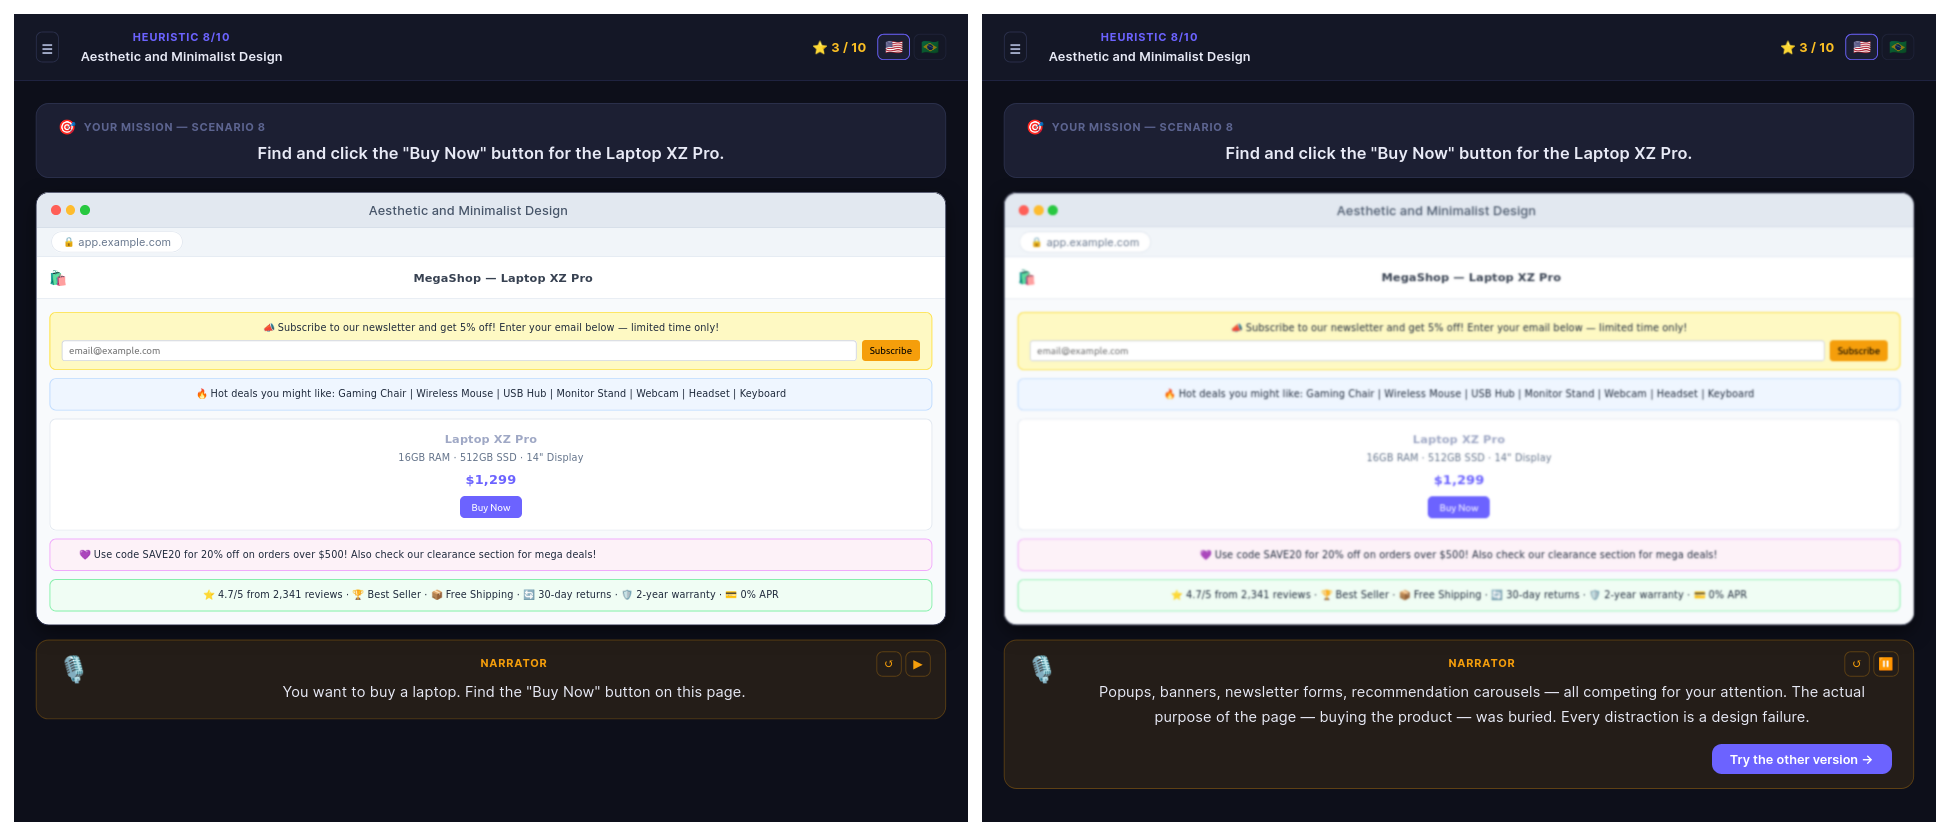
\includegraphics[width=.95\textwidth]{figures/h8-bad-scenario-after-and-before.png}}
{Two side-by-side screenshots of the bad scenario for heuristic 8 (Aesthetic and Minimalist Design). On the left, the player enters the scenario: the mission ``Find and click the Buy Now button for the Laptop XZ Pro'' appears at the top, above a cluttered shop interface with overlapping yellow newsletter banners, recommendation carousels of unrelated products, deal labels, and prices that obscure the actual product. The narrator at the bottom says: ``You want to buy a laptop. Find the Buy Now button on this page.'' On the right, the same interface is shown after the task is completed; the narrator now comments: ``Popups, banners, newsletter forms, recommendation carousels --- all competing for your attention. The actual purpose of the page --- buying the product --- was buried. Every distraction is a design failure.''}
\caption{Bad scenario for heuristic 8 (Aesthetic and Minimalist Design): the player's mission and the cluttered interface they meet (left), and the narrator's commentary after the task is completed (right).}
\label{fig:h8-bad}
\end{figure}

\begin{figure}[ht]
\centering
\pdftooltip{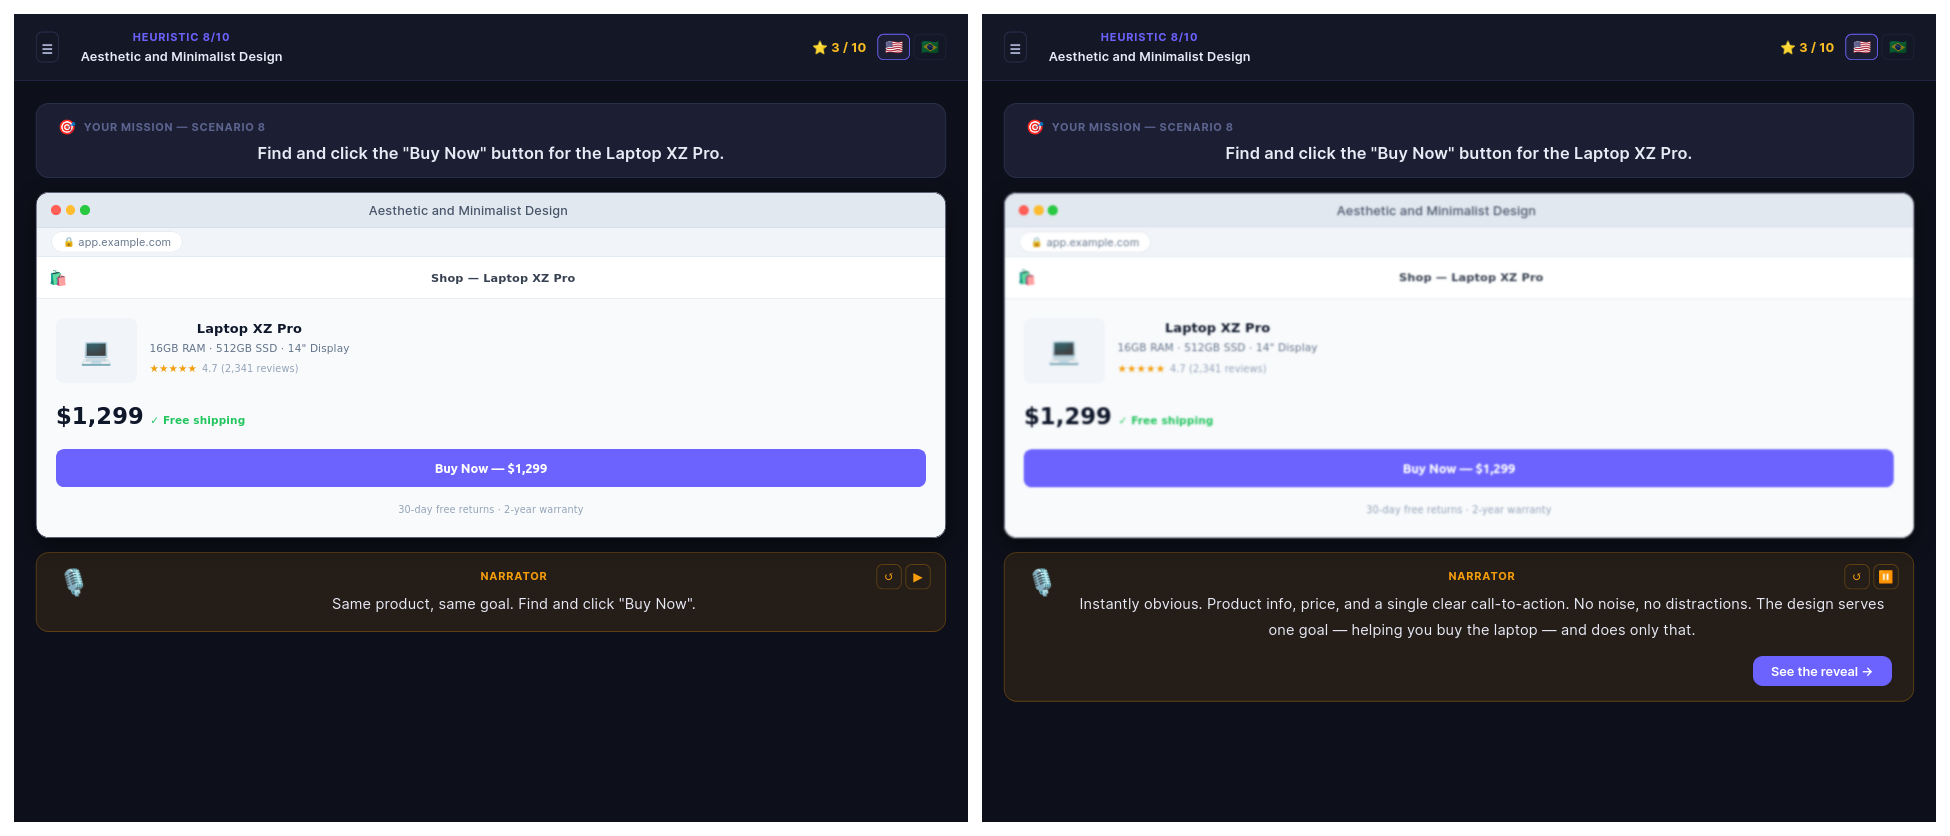
\includegraphics[width=.95\textwidth]{figures/h8-good-scenario-after-and-before.png}}
{Two side-by-side screenshots of the good scenario for heuristic 8 (Aesthetic and Minimalist Design). On the left, the player enters the scenario with the same mission ``Find and click the Buy Now button for the Laptop XZ Pro'' at the top, but the interface below is now minimal: a single product card for the Laptop XZ Pro showing its name, specifications (16 GB RAM, 512 GB SSD, 14-inch display), a 4.7-star rating, the price (\$1,299) with free shipping, and a single prominent purple ``Buy Now --- \$1,299'' button below. The narrator says: ``Same product, same goal. Find and click Buy Now.'' On the right, the same interface is shown after the task is completed; the narrator now comments: ``Instantly obvious. Product info, price, and a single clear call-to-action. No noise, no distractions. The design serves one goal --- helping you buy the laptop --- and does only that.''}
\caption{Good scenario for heuristic 8 (Aesthetic and Minimalist Design): the same mission in a minimal interface (left), and the narrator's commentary after the task is completed (right).}
\label{fig:h8-good}
\end{figure}

\begin{figure}[ht]
\centering
\pdftooltip{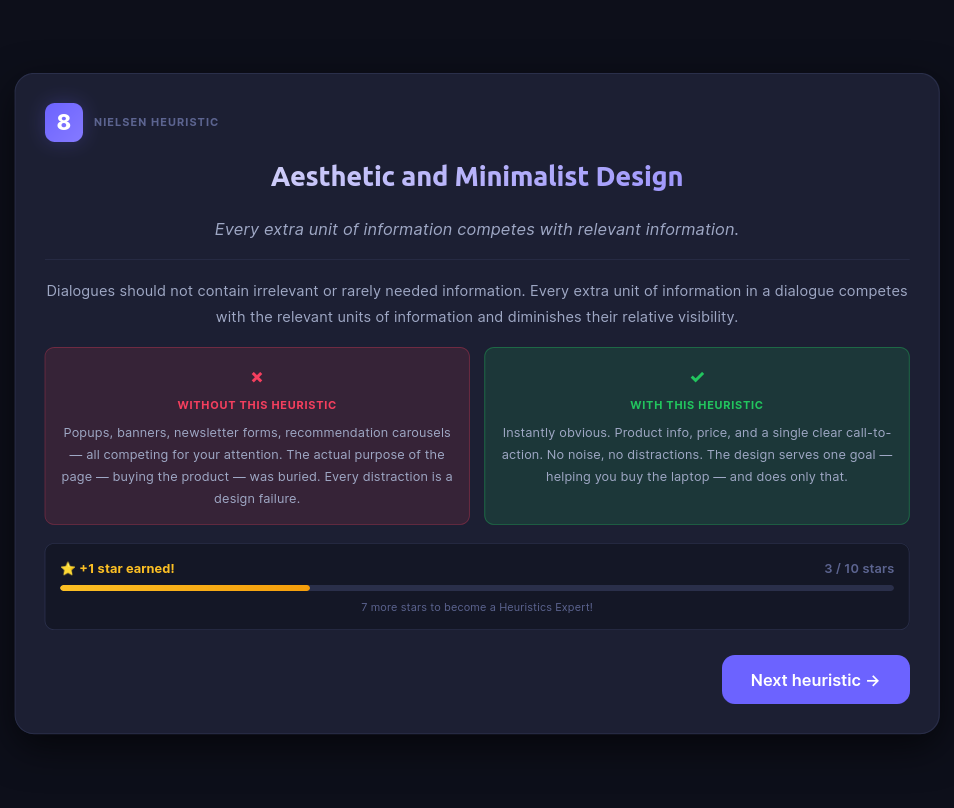
\includegraphics[width=.75\textwidth]{figures/h8-reveal-screen.png}}
{Reveal screen for heuristic 8 (Aesthetic and Minimalist Design). At the top, the heuristic number ``8'' and the label ``Nielsen Heuristic'' precede the heuristic title ``Aesthetic and Minimalist Design''. Below, the tagline reads ``Every extra unit of information competes with relevant information.'', followed by Nielsen's full definition: ``Dialogues should not contain irrelevant or rarely needed information. Every extra unit of information in a dialogue competes with the relevant units of information and diminishes their relative visibility.'' Two side-by-side coloured cards then recap the contrast: on the left, a red ``Without this heuristic'' card explains that popups, banners, newsletter forms, and recommendation carousels competed for the player's attention and buried the actual purpose of the page; on the right, a green ``With this heuristic'' card explains that product info, price, and a single clear call-to-action made the goal instantly obvious. At the bottom, a yellow progress bar indicates ``+1 star earned'' and shows the running total of 3 out of 10 stars, with the message ``7 more stars to become a Heuristics Expert!''. A purple ``Next heuristic'' button sits at the bottom right.}
\caption{Reveal screen for heuristic 8: the heuristic is named and defined, the contrast between the two scenarios is recapped, and a star is awarded.}
\label{fig:h8-reveal}
\end{figure}

\subsection{The ten heuristics}

The ten heuristics covered by the game follow the consolidated formulation by Nielsen~\cite{nielsen1994heuristic,nielsen2024tenheuristics}. Each heuristic is paired with a concrete, self-contained task that can be carried out by the player in a few clicks within a single screen. The bad and the good scenario for the same heuristic use the same task, but the interface around it is intentionally redesigned so that the contrast between violating and respecting the heuristic is directly visible in the interaction. Table~\ref{tab:heuristics} lists the heuristics in the order in which they appear in the game, the task used in each pair of scenarios, and the specific design contrast between the violating and the compliant interface.

{
\footnotesize
\setlength{\tabcolsep}{4pt}
\begin{longtable}[c]{c|p{2.3cm}|p{2.5cm}|p{4.0cm}|p{4.0cm}}
  \caption{The ten Nielsen heuristics, the concrete task used in each pair of scenarios, and the design contrast between the violating (bad) and the compliant (good) interface.}
  \label{tab:heuristics}\\
  \hline
  \textbf{\#} & \textbf{Heuristic} & \textbf{Task} & \textbf{Bad scenario} & \textbf{Good scenario} \\
  \hline
  \endfirsthead

  \multicolumn{5}{l}{\textit{Table~\thetable\ --- continued from previous page}}\\
  \hline
  \textbf{\#} & \textbf{Heuristic} & \textbf{Task} & \textbf{Bad scenario} & \textbf{Good scenario} \\
  \hline
  \endhead

  \hline
  \multicolumn{5}{r}{\textit{Continued on next page}}\\
  \endfoot

  \hline
  \endlastfoot

  1 & Visibility of System Status & Send a message to a friend about dinner tonight. & No feedback while the message is sending; the user cannot tell whether it went through. & A progress bar followed by a ``Message delivered'' confirmation keeps the user informed at every step. \\
  \hline
  2 & Match Between System and the Real World & Save the document before closing. & Buttons labelled ``Serialize \& commit to persistent storage layer'' and ``Discard volatile in-memory state'' force the user to decode technical jargon. & Plain-language labels such as ``Save'' and ``Discard changes'' use the vocabulary people actually think in. \\
  \hline
  3 & User Control and Freedom & Exit an accidentally opened upgrade wizard without completing the upgrade. & No cancel, close, or back option on the first step --- the user must either complete the upgrade or abandon the session. & Multiple clearly marked exits (a close button, a cancel link on every step, and a confirmation dialog) let the user leave at any point. \\
  \hline
  4 & Consistency and Standards & Navigate through all four checkout steps. & Navigation buttons change label (``Proceed'', ``Go on'', ``Continue'') and position from step to step, forcing the user to re-learn the interface at every screen. & Identical ``Back'' and ``Next'' buttons in the same position on every step. \\
  \hline
  5 & Error Prevention & Delete the account from settings. & A single click permanently deletes the account, with no warning or confirmation. & Several protective layers --- a de-emphasised button, a warning dialog, a type-to-confirm field, and an acknowledgement checkbox --- prevent accidental deletion. \\
  \hline
  6 & Recognition Rather Than Recall & Make the word ``important'' bold in a document. & Toolbar buttons are labelled only ``1'', ``2'', and ``3'', with no indication of what they do; the user has to memorise or guess. & Visible, familiar formatting controls let the user recognise the correct action immediately. \\
  \hline
  7 & Flexibility and Efficiency of Use & Mark all three unread notifications as read. & Each notification must be dismissed individually; no bulk action is available. & A single ``Mark all as read'' action handles the task, while individual dismiss options remain available for granular control. \\
  \hline
  8 & Aesthetic and Minimalist Design & Find and click the ``Buy Now'' button for the Laptop XZ Pro. & Popups, banners, newsletter forms, and recommendation carousels compete for attention and bury the actual goal of the page. & A clean layout shows only the product, the price, and a single clear call-to-action. \\
  \hline
  9 & Help Users Recognise, Diagnose, and Recover from Errors & Fix the form error and complete registration. & A generic message ``Error 422: Unprocessable Entity'' tells the user nothing about which field is wrong or how to fix it. & Inline error messages highlight the exact field and explain the specific problem (for example, ``Password must be at least 8 characters''). \\
  \hline
  10 & Help and Documentation & Enable Two-Factor Authentication in Security Settings. & Options are labelled only by acronym (``2FA'', ``TOTP'', ``FIDO2''), with no explanation or links to documentation. & Each option carries a plain-language description and an inline information tooltip, with a recommended choice highlighted. \\
\end{longtable}
}

The interfaces used in the bad and good scenarios are not static mock-ups: they are interactive components that the player operates with real clicks, typing, and navigation. This was a deliberate design choice, so that the difference between violating and respecting a heuristic is felt through the interaction rather than read as a description.

\subsection{Narration and gamification}

A narrator accompanies the player throughout the game. Before each scenario, the narrator restates the goal and primes the player's attention; after the task is completed, the narrator returns with a short commentary that names what just happened in the interface in terms of the heuristic in play. Each piece of narration is delivered both as on-screen text and as a voice-over, with the audio falling back silently to text if it cannot be played; each track also exposes pause, resume, and replay controls. The artefact does not include an in-game mute toggle: silencing the narration entirely is delegated to the device or browser volume. The narrator is framed in the design as a focusing and reflection device, not as an authority figure who tells the player whether a choice was correct.

A few lightweight gamification elements sit on top of the educational content. A star is awarded after each reveal screen, and a small ``X out of 10'' indicator in the top bar shows the running progress. A collapsible side panel lists the ten heuristics and the player's status on each, so the player can review what has already been covered. A celebratory closing screen, reached after the tenth star, greets the player as a ``heuristics expert'' before the final results screen. These elements are intended as engagement scaffolding --- helping the player stay focused and complete the full sequence in one session --- rather than as a separate learning mechanism.

\subsection{Scope of the design}

A few features were deliberately left out of the artefact, and it is worth naming them explicitly. With ten heuristics to cover, each in a pair of scenarios, the design prioritised completability within a single classroom session over depth per heuristic: richer challenge mechanics --- failure states, scoring, branching paths, longer narration --- would have multiplied the time per heuristic and made the total session impractical for typical class use. The game therefore does not adapt to the player: all participants see the same ten heuristics in the same order, and there is no adaptive difficulty. The game also does not assess learning in a quiz-style way. The bad scenarios do produce in-task friction --- attempts that do not advance the goal until the player works around the violation --- but the player is never asked to identify the heuristic on their own, and there is no scoring of decisions. There is no collaborative or social mode; the experience is single-player and single-session, and replaying the game shows the same content. The artefact is intentionally a content-delivery and reflection-scaffolding device that complements an instructor, rather than a stand-alone teaching system or an assessment instrument.

% \section{User Study Methodology}
\label{sec:method}

% \subsection{Study type and participants}

This work is an experience report on the design and qualitative evaluation of a web-based educational game that supports the understanding of Nielsen's ten heuristics. The artifact was analyzed by HCI students, professors, and industry professionals, who were reached via convenience sampling. 

% deployed in two complementary settings. The first was an HCI evaluation course at a Brazilian university (omitted for double-blind review), where the course instructor applied the game during regular class time, after the ten heuristics had already been introduced through the standard course content. This setting closely mirrors the intended classroom use of the artefact, in which the game supports the understanding of heuristics that the instructor has just taught. The second setting was remote participation reached through the research team's network, which broadens the range of participant profiles beyond the host course.

Participants formed a mixed audience of undergraduate and graduate students from computing-related programs, with additional professionals and researchers reached through the wider network. Prior familiarity with Nielsen's heuristics varied among participants: some had been introduced to them this semester, while others encountered them for the first time through the game. This variation is captured by a dedicated item in the demographic questionnaire so that responses can be read against prior exposure when relevant. Recruitment was non-probabilistic; no personally identifiable information was collected. The final sample includes $N = 30$ responses; no entries were removed during the data cleaning (see Section~\ref{sec:results}).

\subsection{Procedure}

Each participant followed the same sequence. They opened the game in a web browser, played end-to-end through the ten heuristics, and then clicked through to a linked questionnaire from the game's final results screen \footnote{The questionnaire was administered through Google Forms in Portuguese, the language approved by the ethics committee for this .}. Its first page presented the informed-consent statement, which had to be accepted before continuing. The remaining pages contained five categorical demographic questions and five open-ended questions about the participant's experience.

The demographic questions covered current role, age, primary area of work or study, prior familiarity with Nielsen's heuristics, and practical experience with HCI or usability evaluation. The open-ended questions were related to (a) overall appreciation of the game, (b) perceived support to understand the heuristics, (c) the effect of gamification and narration on experience and learning, (d) negative points and suggested improvements, and (e) further comments. Responses were automatically collected in a linked spreadsheet available exclusively to the research team.

% The questionnaire deliberately omits Likert-style agreement scales. This choice reflects two design constraints. The expected sample size is small, which limits what numeric scales can reveal at this scale. The research question also targets the mechanisms behind perceived support --- something better captured by open-ended responses that participants are free to phrase in their own terms.

\subsection{Data analysis}

The open-ended responses were analyzed through qualitative content analysis \cite{bardin2011}, following the four-step procedure adopted for this study. First, the responses were screened for engagement: entries that were obviously not engaged with the question (for instance, single-character or filler responses) would be removed at this step. Second, the demographic answers were summarized through charts, each accompanied by a textual description so that the argument can be followed without consulting the figure. Third, the open-ended responses were grouped by question and inductively clustered into themes: similar responses were brought together and named, with cross-participant comparisons to identify shared patterns rather than listing individual answers. Fourth, the themes were exemplified through anonymized excerpts, with participants identified only as $P_1, P_2, \ldots$; where context matters for a given quote, a short demographic tag is added (for example, ``$P_3$ (graduate student, computer science, no prior familiarity with the heuristics)'').

\subsection{Ethical considerations}
\label{sec:ethics}

This experience report respects the Brazilian regulatory framework for research involving human participants. The study is part of a project approved by the host university's Research Ethics Committee, approved under CAAE number (omitted for double-blind review).

Participation was voluntary, non-remunerated, and could be withdrawn at any moment without consequence. Before answering the questionnaire, each participant read an Informed Consent Form, describing the details of the research, and consent had to be explicitly given before any further questions could be answered.

% \section{Cuidados Éticos}
\label{sec:ethics}

This experience report respects the Brazilian regulatory framework for research involving human participants. The study is part of an umbrella project at the host university's Research Ethics Committee (Comit\^{e} de \'{E}tica em Pesquisa, CEP), approved under CAAE (omitted for double-blind review), and follows the requirements of CNS Resolutions 466/2012 \cite{cns466_2012}, 510/2016 \cite{cns510_2016}, and 674/2022 \cite{cns674_2022}, as well as Operational Norm 001/2013 \cite{cns_no001_2013}.

\subsection{Participant consent and rights}

Participation was voluntary, non-remunerated, and could be withdrawn at any moment without consequence. Before answering the questionnaire, each participant read an Informed Consent Form (\emph{Termo de Consentimento Livre e Esclarecido}, TCLE) approved by the ethics committee. The form described the purpose of the research, the activities involved, the foreseen risks and benefits, the right to withdraw at any time, the team's contact information, and the way the collected data would be handled. Consent had to be explicitly given before any further question could be answered.

The risks were considered minimal. The activity is comparable to using a website and answering a few open-ended reflection questions, and could cause at most some discomfort from the time spent or fatigue from reading. No clinical, physical, or invasive procedures were involved. The foreseen benefits are indirect: participants contributed to research on the teaching of Nielsen's heuristics and to the refinement of an educational artefact for the HCI community.

\subsection{Anonymity}

No personally identifying information was collected at any point. The demographic questions are all categorical (role, age range, area, prior familiarity with the heuristics, and practical experience with HCI evaluation), and no names, emails, IP addresses, or other identifiers are recorded by the game or by the questionnaire. In the analysis and in this paper, participants are referred to only as $P_1, P_2, \ldots$, with a short demographic tag added when context for a quote is needed. No participant images are used in this paper.

\subsection{Data protection (LGPD)}

The processing of participant data follows the Brazilian General Data Protection Law \cite{lgpd2018}. Because the questionnaire collects only categorical and self-reported responses with no direct identifiers, the resulting dataset is pseudonymous by design. Responses are stored in a spreadsheet linked to the form, with access restricted to the research team. Aggregate analyses and anonymised excerpts are used for academic communication; the raw data are not redistributed. The data are retained for five years from collection, in line with the consent form, and are used only for the purposes described to participants.

% \section{User Study Results  (NEW VERSION!!!)}
\label{sec:results}

The next subsections present the results obtained.

\subsection{Participants}
\label{sec:results:participants}

The questionnaire was answered by $N = 31$ participants over a six-day window in May 2026. All responses were substantive, so no entries were removed during data cleaning. % The three figures that follow summarise the sample. Each is described in prose so the argument can be followed without consulting the chart.

Figure~\ref{fig:demographics-role-area} pairs the current role with the primary area of study or work. The role question allowed more than one selection, since some participants combine study and professional practice. Most respondents were students --- 16 undergraduates, 8 master's students, and 3 doctoral students. Four were professors or researchers. Five of the student respondents additionally reported professional experience outside the university; this appears in the role chart as a secondary multi-select pick rather than as a separate primary category. The area distribution is heavily skewed: 25 of the 31 participants come from Computer Science or Software Engineering, with 3 from Design or UX, 1 from Information Systems, and 2 from other technology areas.

\begin{figure}[ht]
\centering
\pdftooltip{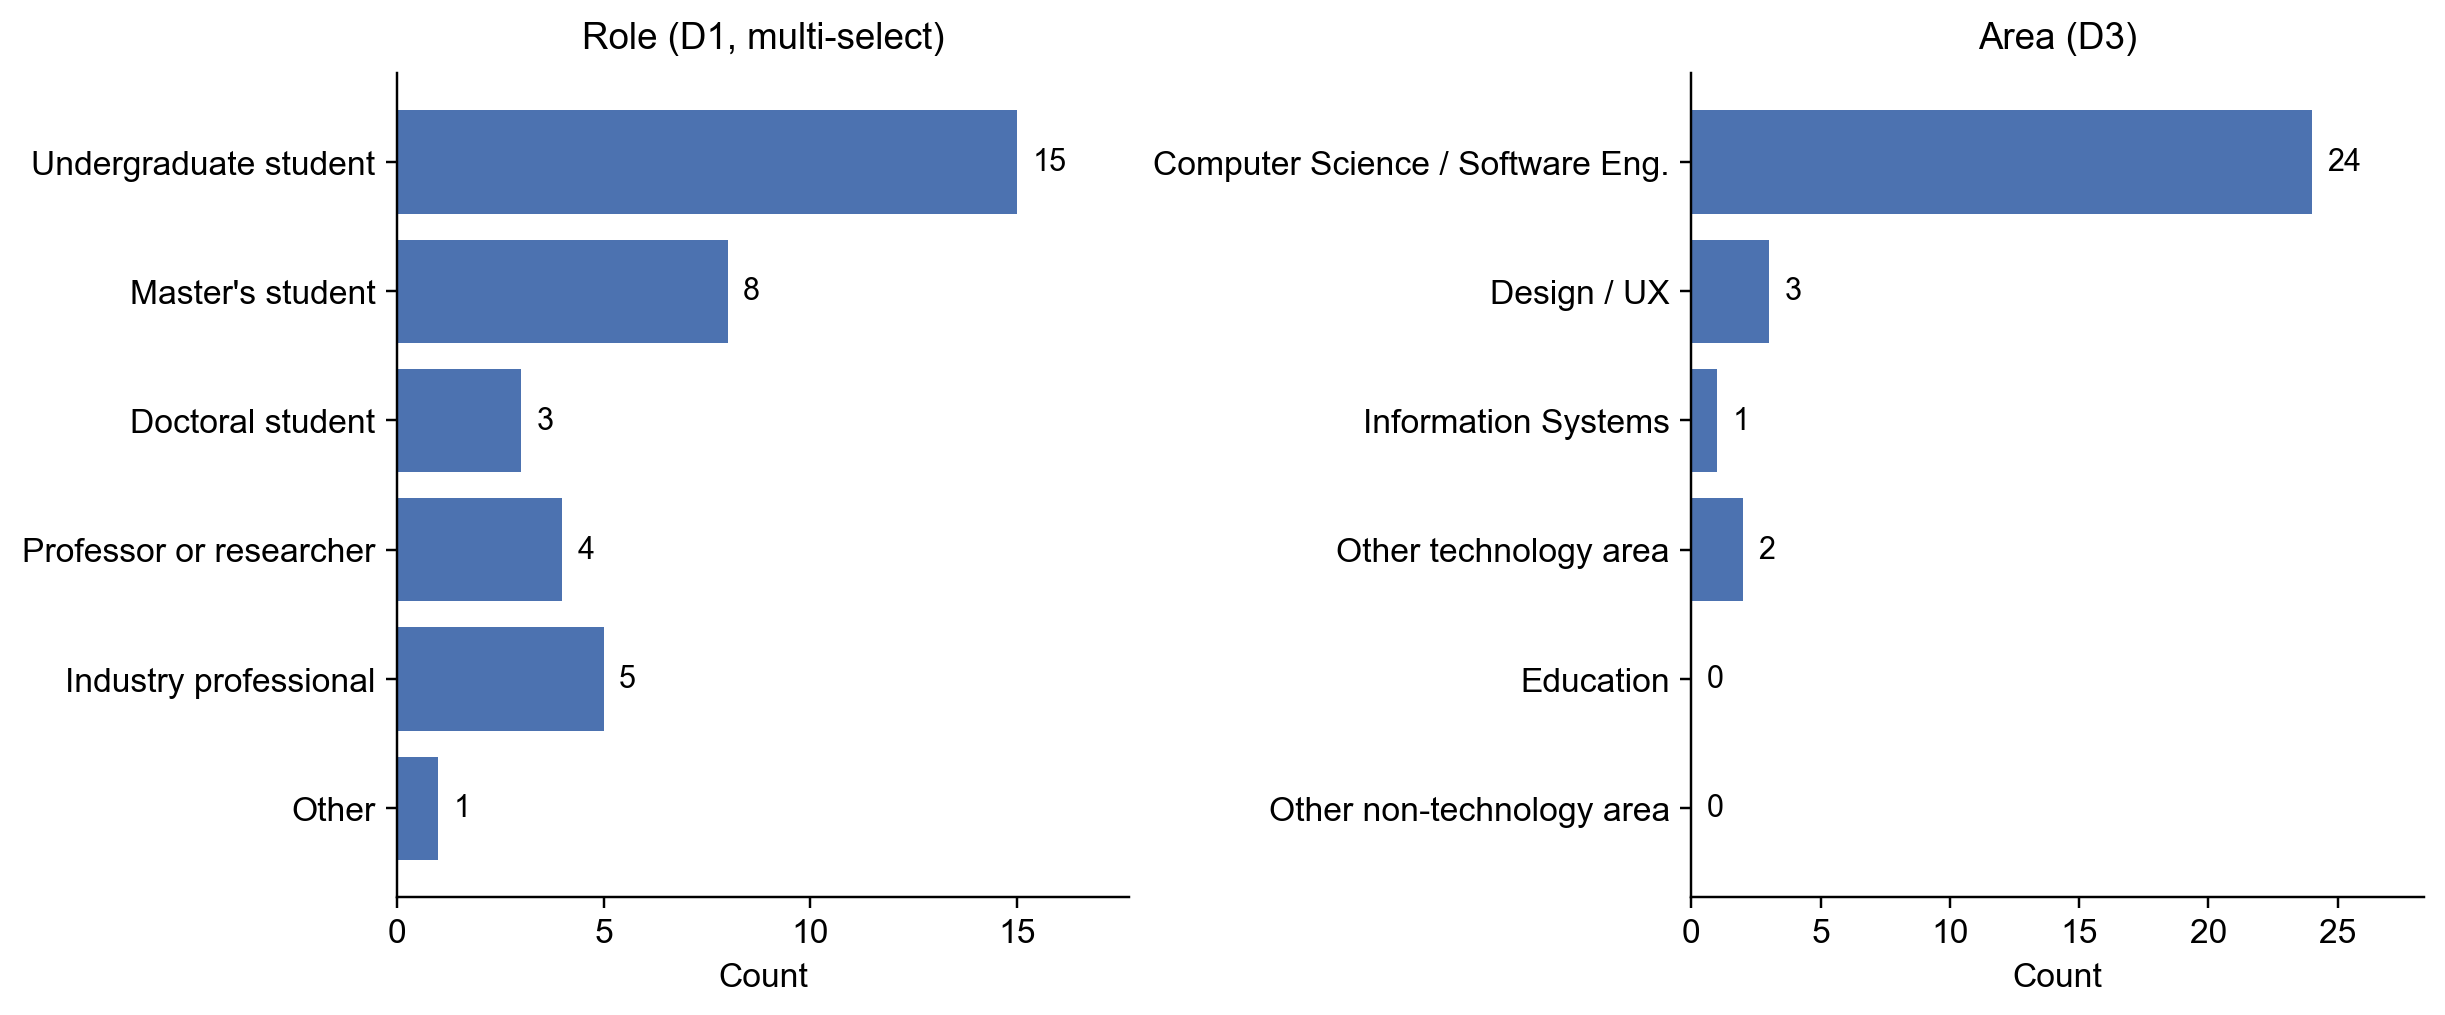
\includegraphics[width=.95\textwidth]{figures/demographics-role-area.png}}{Two horizontal bar charts side by side. The left chart shows the count of selections for each role option: 16 for undergraduate student, 8 for master's student, 3 for doctoral student, 4 for professor or researcher, 5 for industry professional, and 1 for ``other''. The role question was multi-select, so several participants selected more than one role; the ``industry professional'' count overlaps with student categories rather than denoting a separate primary group, and the total exceeds the sample size of 31. The right chart shows the count for each area: 25 for Computer Science or Software Engineering, 3 for Design or UX, 1 for Information Systems, and 2 for ``other technology area''.}
\caption{Participant roles (multi-select) and primary areas of study or work.}
\label{fig:demographics-role-area}
\end{figure}

Figure~\ref{fig:demographics-age} shows the age distribution. Ages span from 18 to 52, with a median of 24. Sixteen participants fall in the 18--24 range, 12 in the 25--34 range, 2 in the 35--44 range, and 1 in the 45--54 range. The sample skews young, which is consistent with the dominant student profile reported above.

\begin{figure}[ht]
\centering
\pdftooltip{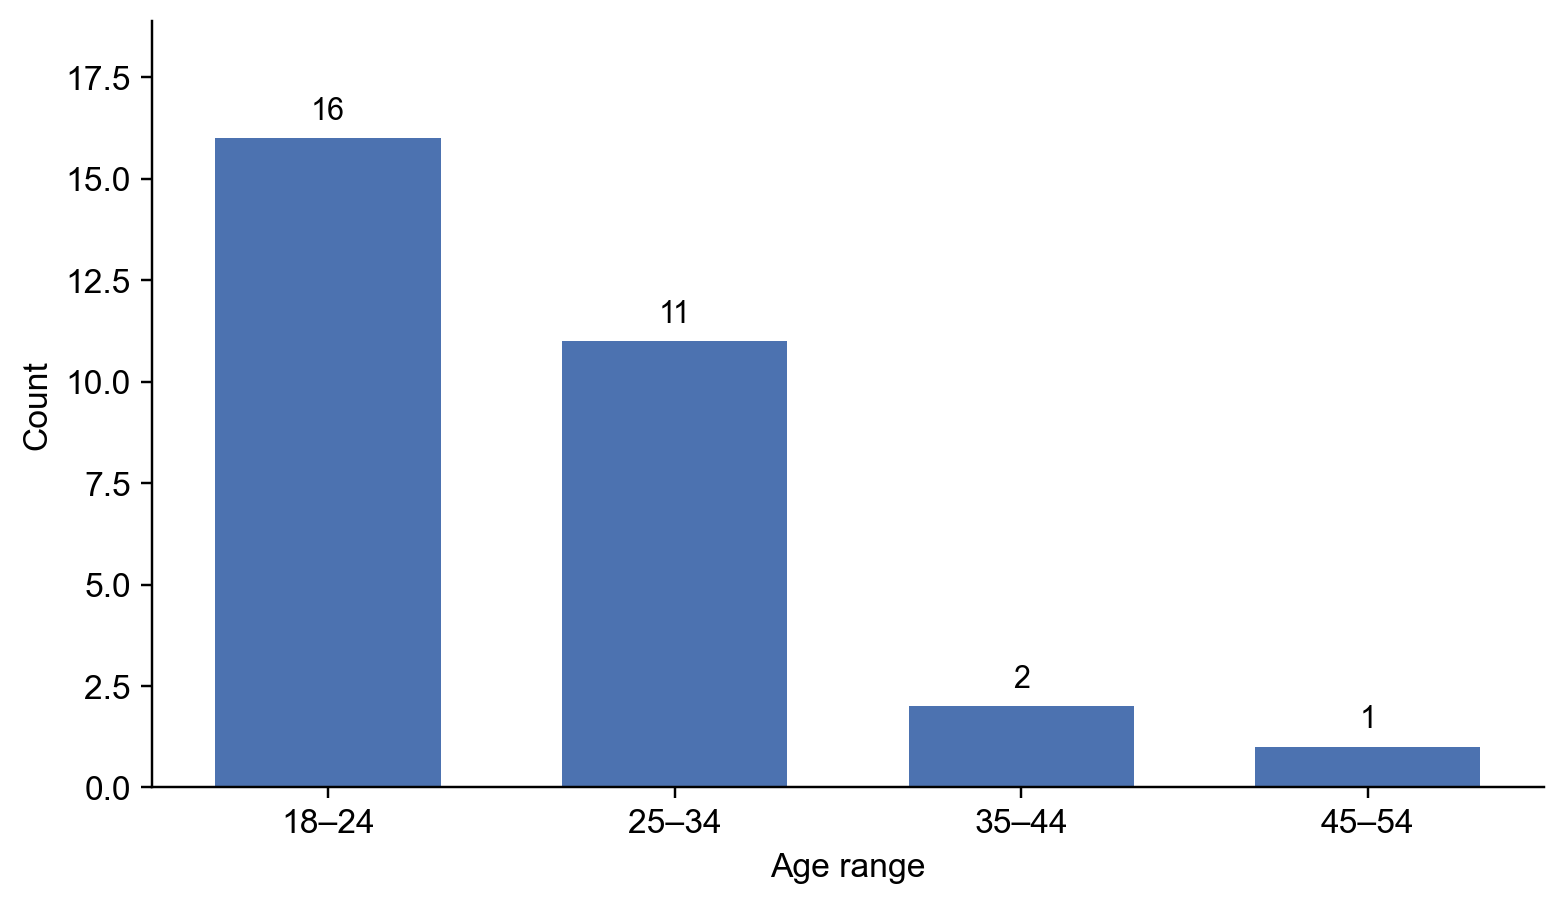
\includegraphics[width=.7\textwidth]{figures/demographics-age.png}}{A histogram of participant ages with four age-range bins on the horizontal axis: 18--24, 25--34, 35--44, and 45--54. The bars have heights 16, 12, 2, and 1, respectively. The distribution is right-skewed, with most participants in the youngest two bins.}
\caption{Distribution of participant ages across four age ranges.}
\label{fig:demographics-age}
\end{figure}

Figure~\ref{fig:expertise-profile} pairs prior familiarity with Nielsen's heuristics with practical experience in HCI or usability evaluation. Both scales are ordered from novice at the top to expert at the bottom. On the familiarity scale, 17 participants reported limited prior familiarity with the heuristics, 7 reported moderate familiarity, 6 knew them well, and 1 had already used them in projects or evaluations. On the practical-experience scale, 8 reported no practical experience, 13 reported little experience limited to coursework, 6 reported some experience in academic projects, and 4 reported regular practice in their professional or research work.

\begin{figure}[ht]
\centering
\pdftooltip{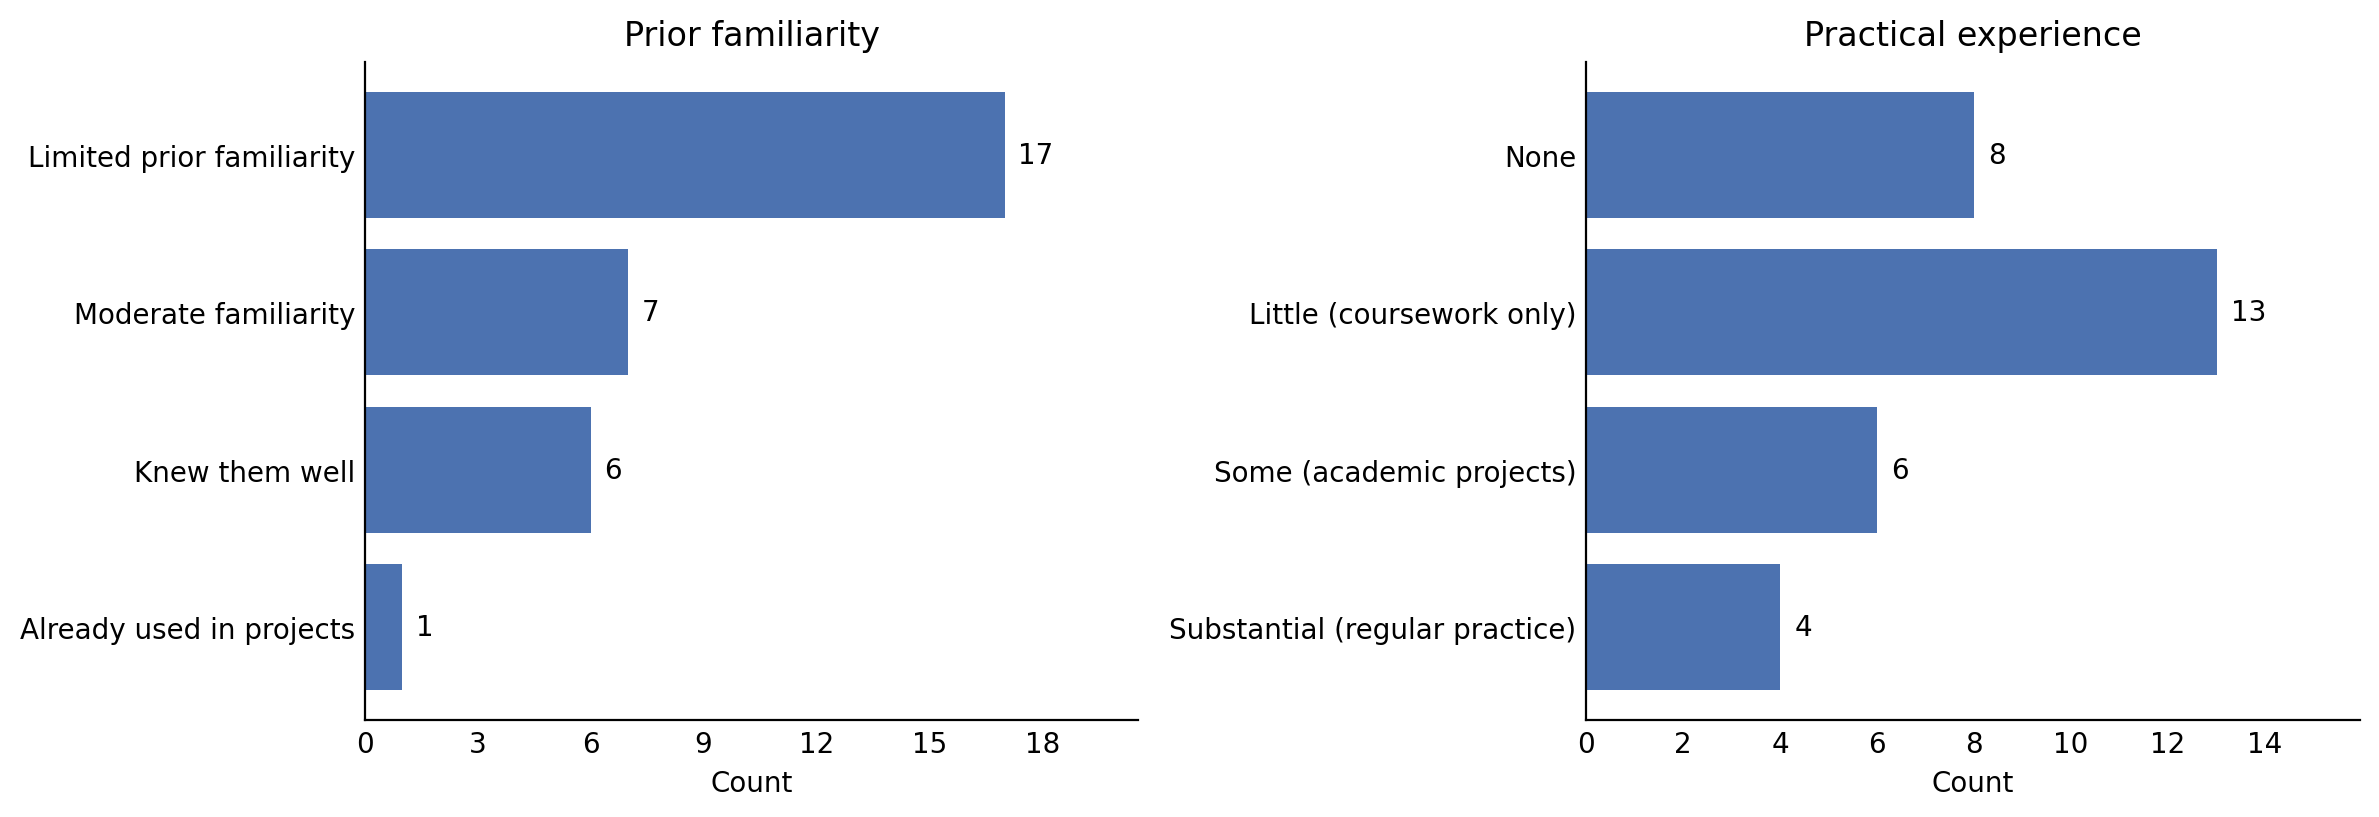
\includegraphics[width=.95\textwidth]{figures/expertise-profile.png}}{Two horizontal bar charts side by side, both ordered from novice at the top to expert at the bottom. The left chart shows the count for each level of prior familiarity with Nielsen's heuristics: 17 for ``limited prior familiarity'', 7 for ``moderate familiarity'', 6 for ``knew them well'', and 1 for ``had already used them in projects or evaluations''. The right chart shows the count for each level of practical experience with HCI or usability evaluation: 8 for ``none'', 13 for ``little, only in coursework'', 6 for ``some, in academic projects'', and 4 for ``substantial, in regular professional or research practice''.}
\caption{Prior familiarity with Nielsen's heuristics and practical experience with HCI or usability evaluation.}
\label{fig:expertise-profile}
\end{figure}

The sample is therefore dominated by computing students, most with limited prior familiarity with the heuristics. A smaller group --- designers, professors, and participants with more practical HCI experience --- provides a critical contrast in the qualitative analysis that follows. Participant identifiers ($P_1$ through $P_{31}$) are anonymous and follow the order in which the responses were received.\footnote{Original responses were written in Portuguese. Quotes shown in this section were translated by the authors; the AI-tool disclosure for translation is provided in the Acknowledgments.}

\subsection{Overall appreciation}
\label{sec:results:t1}

Most participants reported a positive overall experience with the game (27 of 31); the remaining four mixed or negative responses are revisited together in Section~\ref{sec:results:t6}. The reasons given for liking the game clustered into a few recurring themes.

The most common reason was \textbf{didactic clarity}. Several participants described the game as \textit{``didactic''} or \textit{``informative''}, and as a way to \textit{``transform theory into practice''} ($P_{19}$, undergraduate, Information Systems). A second recurring theme was that \textbf{the scenarios mirror real-world frustrations}. $P_1$ (master's, limited prior familiarity) noted that the game \textit{``showed problems that really happen and that companies do nothing to fix''}. $P_{16}$ (undergraduate, also industry professional) reframed this as a pedagogical strategy: \textit{``the game gives you a first-person perspective; suffering to learn is a good tactic so you do not make the same mistakes again''}.

\subsection{Perceived support for understanding}
\label{sec:results:t2}

When asked how the game supported their understanding of Nielsen's heuristics, participants identified three mechanisms that together account for most of the perceived support.

The first and most-cited mechanism is the \textbf{paired contrast} between the violating and the compliant scenarios. Nine participants named the contrast as the single most important aspect of the game. $P_1$ wrote that \textit{``the comparison between the examples was the most distinguishing feature; showing first the wrong version and then the right one helped me a lot''}. $P_{12}$ (master's, limited prior familiarity) made the same point in different words: \textit{``what helped me the most was the way the game first showed a messy scenario and right after a correct one''}. The same mechanism is named by $P_6$, $P_{11}$, $P_{15}$, $P_{16}$, $P_{21}$ and $P_{31}$, often using the words \textit{``error and correct''}, \textit{``worse versus better''}, or \textit{``without and with''} --- the same vocabulary the game itself uses on the reveal screen.

The second mechanism is the \textbf{interactive nature of the scenarios}. Participants treated \textit{``practical examples''} and \textit{``interactive interfaces''} as distinct from a static contrast: doing the task in the violating interface made the heuristic concrete. $P_{14}$ (professor, Design/UX, knew the heuristics well) summarized this clearly: \textit{``the fact that the interfaces are interactive contributed without doubt to a better understanding; it let me experience how the design is actually an obstacle for the user''}. $P_9$ (master's) gave the most specific illustration: ``the interactive part --- sending the message and feeling the impact of thinking it had been lost, for example''. The episode refers to the bad scenario for Heuristic~1 (Visibility of System Status), in which the player sends a message to a friend in an online chat and receives no feedback while the message is being sent. The same emphasis on interactivity as the source of understanding appears in $P_{10}$, $P_{13}$, $P_{17}$, $P_{22}$, $P_{23}$, and $P_{27}$.

The third mechanism is the \textbf{naming of the concept on the reveal screen}. For participants with limited prior familiarity with the heuristics, the reveal step is where the practical experience is named and labeled. $P_5$ (master's, limited prior familiarity) put it directly: \textit{``I did not even know these concepts had names like that''}. $P_{24}$ (undergraduate, also industry professional, moderate familiarity) added that \textit{``seeing each heuristic explained and named separately was useful; it added to what I already knew''}.

Several participants made the comparison with traditional reading explicit. $P_{30}$ articulated this most fully: \textit{``I would have taken longer to understand by reading a fancy definition on its own; this was a good combination of learning and entertainment. It is a more active method of learning than just reading, which is a more passive way.''} One participant offered a mild dissent: $P_7$, who did not find the game very supportive, still acknowledged that \textit{``at least we had some examples of errors and successes according to Nielsen's heuristics''}.

\subsection{Gamification and narration}
\label{sec:results:t3}

When asked about the effect of gamification (stars, progress bar, and the ``Heuristics Expert'' closing screen) and narration on their experience and learning, participants' responses split cleanly into two sub-themes, which we present separately because the responses diverge in direction.

For \textbf{gamification}, thirteen participants reported a positive effect on focus or motivation. $P_1$ noted that the gamification \textit{``helped me stay focused and more immersed; it stopped being something boring and only theoretical''}. $P_{24}$ added that \textit{``gamifying helped me hold my attention and made the learning process more satisfying''}. A separate group of six respondents singled out the progress bar as helpful while saying the stars and the Expert screen did not affect them. $P_2$ wrote that \textit{``the progress bar gave me a sense of arriving somewhere; the stars did not influence me or motivate me''}. $P_{31}$ gave the underlying reason: \textit{``I liked the progress bar; I hate it when something does not tell you how long it will be and seems to never end''}, framing the bar as a defense against the experience of an open-ended task. Three participants reported no effect from gamification at all ($P_{13}$, $P_{29}$, $P_{30}$). The remaining critique was structural: $P_6$ (professor) said gamification \textit{``helped only superficially, since there was practically only one path to follow and it was not possible to lose points''}; $P_7$ extended this into a call for \textit{``a real gamification with scoring and rewards''}.

For \textbf{narration}, ten participants described it as helping them focus or recognise the heuristic in action. $P_8$ (master's, limited prior familiarity) gave the sharpest example: \textit{``in some cases without the heuristic I got irritated by the lack of pattern, and the narration helped me understand that this was exactly what was being demonstrated''}. $P_{14}$ added that \textit{``the narration contributed to understanding and to staying focused on the activity''}. $P_{31}$ named a distinct mechanism --- the narration as a way of taking the reading work off the player so they can engage with the practical task: \textit{``the most interesting part for me was the narration; constantly reading non-practical aspects makes you feel lazy when you have to start doing something practical, and having the narrator do that work brings down a barrier so you can focus on what matters''}. Four participants reported the opposite effect. $P_{18}$ wrote that the narration \textit{``bothered me a bit''} and that a button to silence it was missing; $P_{20}$ and $P_{22}$ raised similar points about volume control and distraction from reading. $P_{10}$ accepted the narration but commented that it \textit{``could be a little less robotic''}.

\subsection{Reported issues and suggestions}
\label{sec:results:t4}

When asked about negative points and improvements, and in optional general comments at the end of the questionnaire, three recurring patterns appear across the responses.

The most consistent pattern is a \textbf{wish for the player to be able to fail or to choose}. Five participants asked for an explicit way to be wrong or for more challenge. $P_2$ suggested that the user should try to identify which heuristic applies before the game reveals it; $P_7$ argued that without the possibility of error there is no need to reason, which makes the experience tedious; $P_8$ proposed losing stars or lives on mistakes; $P_{18}$ and $P_{25}$ asked for a more interactive format with real decisions. The wording differs but the underlying request is the same: a recognition step that the player completes before the reveal screen.

The second pattern is \textbf{narration ergonomics}. Beyond the mixed reception reported in Section~\ref{sec:results:t3}, four participants pointed to concrete affordances: $P_5$ asked that the audio not play automatically; $P_{18}$ and $P_{20}$ asked for a mute or volume control; $P_9$ noted that some narration tracks were long enough to feel like watching a video. These are inexpensive to address.

The third pattern is a \textbf{desire for more depth} and a small set of one-off suggestions. $P_{16}$ proposed adding a second activity per heuristic to support fixation and $P_6$ suggested that some scenarios could be replaced by more realistic variants. A scattered set of further comments touched on small interface details and atmosphere --- including $P_{17}$'s suggestion that the game open with a light-hearted warning about being intentionally frustrating at first --- but did not cluster within a shared theme.

\subsection{Critical reception}
\label{sec:results:t6}

Four of the thirty-one responses read the artefact more as a guided demonstration than as a game proper. The three quoted below illustrate the range of how this position was expressed. $P_2$ (master's, designer, knew the heuristics well) expected to be challenged and instead experienced \textit{``almost a guided tour through the heuristics''}. $P_7$ (undergraduate) was more explicit: \textit{``there is no aspect of it that resembles a game''}, because \textit{``the user cannot make mistakes and there is no incentive to reason about the answer''}. $P_{30}$ (undergraduate, limited prior familiarity) reached the same conclusion through a different route: \textit{``as a game, no --- in my experience this is a demonstration of how user experience can be done badly, and the corresponding solutions''}.

We return to this tension, and to the related calls for a recognition step or a scoring layer surfaced in Section~\ref{sec:results:t4}, in the discussion of theme 4 in Section~\ref{sec:discussion}.

% \section{Discussion}
\label{sec:discussion}

The qualitative data lets us address the research question directly: in what ways does the paired-scenario game support participants' understanding of Nielsen's heuristics, and how do the surrounding design choices --- narration and light gamification --- affect that support? Four themes recur across the responses, and we discuss each in turn before stating the limitations of the study.

The first theme is that the paired bad/good contrast, combined with the interactive nature of the scenarios, is the mechanism participants most often name when explaining how the game supported their understanding (Section~\ref{sec:results:t2}). This pattern fits an experiential-learning reading of the activity: the player has a concrete encounter with a violating interface, then with a compliant one, and the reveal screen labels the abstract concept that explains the contrast. The sequence operationalises the move from concrete experience to abstract conceptualisation described by Kolb \cite{kolb1984experiential}, and the participants' own language --- $P_{30}$'s ``a more active method of learning than just reading, which is a more passive way'' --- mirrors the active-learning literature \cite{bonwell1991active,freeman2014active}. The contrast itself, named by participants as ``error and correct'' or ``worse versus better'', is what gives the abstract definition something concrete to attach to.

The second theme is that gamification operates as engagement scaffolding rather than as a separate learning mechanism. Participants who said gamification helped them did so by referring to focus, motivation, or the wish to finish the sequence --- not to understanding the heuristics. Several participants explicitly singled out the progress bar as helpful while reporting that the stars and the closing screen did not affect them ($P_2$, $P_5$, $P_{14}$, $P_{22}$, $P_{23}$). Two participants critiqued the gamification more structurally for not introducing a real challenge ($P_6$, $P_7$). The reading we take from this is that progress tracking carried most of the engagement value, and that the achievement layer is the most easily revised part of the design with little expected cost to the support reported in Section~\ref{sec:results:t2}.

The third theme is that the narration is useful for most participants and costly for some. The narration helped about a third of the sample focus and notice the heuristic in action (anchor: $P_8$). It distracted or frustrated a smaller group, with consistent complaints about the absence of a mute or volume control, the length of some tracks, and the speech style ($P_{18}$, $P_{20}$, $P_{22}$, $P_{10}$). The simplest design response is to add per-track playback controls and to make the audio non-automatic, so that each player can choose the modality that fits their attention style. This is not a question of removing narration, but of letting it be an opt-in rather than an opt-out feature.

The fourth theme is the recurring tension around whether the artefact is a game at all. Several participants ($P_2$, $P_7$, $P_{18}$, $P_{30}$) read it as a guided demonstration rather than as a game proper, on the grounds that there is no failure state and no real decision to be made. This critique is honest and consistent with the design choices reported in Section~\ref{sec:game}: the artefact intentionally avoids assessment, scoring, or branching. The participants' proposal --- that the player be allowed to identify the heuristic before the reveal, or to lose stars on mistakes ($P_2$, $P_8$) --- is the most actionable future-work direction we have. It would shift the artefact from a pure content-delivery device to one that also probes recognition, which is the cognitive step on which novices are reported to struggle \cite{nielsen1992finding,abulfaraj2020detailed}.

Several limitations bound the contribution of this experience report. The sample is small ($N = 30$) and self-selected; recruitment combined a classroom deployment with the research team's network, so the participants who chose to play and complete the questionnaire may have been more receptive to the activity than a random sample would have been. The sample is heavily concentrated in Computer Science and Software Engineering (24 of 30) and includes no participants from Education or from outside technology areas, which limits the generalisability of the findings to other audiences and to formal teacher-led settings. The study collected no pre- or post-test of heuristic knowledge, so the claims rest on self-reported support for understanding rather than on measured learning gains. Finally, the deployment was single-session, so retention is not assessed; a delayed re-evaluation would be a natural next step.

% \section{Final Considerations}
\label{sec:conclusion}

This experience report described the design and the qualitative evaluation of a web-based educational game that supports the understanding of Nielsen's ten heuristics through paired interactive scenarios. The contribution is threefold: the artefact itself, a classroom-applicable procedure for using it in an HCI evaluation course, and a qualitative reading of how a sample of thirty participants described the support the game provided. Participants identified the paired bad/good contrast and the interactive nature of the scenarios as the dominant mechanisms of support, with the reveal screen labelling the concept that links experience to definition. The framing the participants used --- active versus passive, error versus correct, with versus without --- mirrors the experiential and active-learning ideas the artefact was designed around.

The design choices that shape the artefact also shape its limits. With ten heuristics to cover, the absence of a scored failure state and of explicit recognition steps was a deliberate trade-off to keep the total session short enough for classroom use; the bad scenarios still produce real in-task friction, but the player is never asked to commit to identifying the heuristic. The data suggests that this trade was right for the audience studied. The same choices produced the most consistent critique in the data, however: several participants read the artefact as a guided demonstration rather than as a game proper, and asked for the very elements that the design had deferred. The artefact is best understood as a content-delivery and reflection-scaffolding device that complements an instructor, not as a stand-alone teaching system or as an assessment tool.

A short list of next steps follows directly from the participants' feedback. The most cited proposal is to add a recognition-checking mode in which the player attempts to identify the heuristic before the reveal, with stars or lives serving as a real challenge layer. Narration ergonomics --- an in-game mute toggle and shorter, opt-in speech segments --- are inexpensive and would resolve the consistent complaints reported in Section~\ref{sec:results:t4}. A second scenario per heuristic would give players a way to consolidate the contrast, as one participant directly suggested. Beyond the artefact, three larger evaluation steps are open: a delayed re-evaluation that measures retention, a multi-site classroom deployment that broadens the participant profile beyond Computer Science and Software Engineering, and a complementary round in which HCI educators play the game themselves to evaluate it as potential adopters --- a perspective the present study did not capture, since the instructor in the classroom deployment applied the game rather than playing it. We hope these refinements help the artefact continue to support, rather than replace, the work an HCI instructor does in introducing the heuristics to learners.

% \section*{Acknowledgments}

We would like to thank all participants who played the game and shared their experiences by completing the questionnaire.

We wish to note the use of generative AI tools during the preparation of this paper. Claude (Anthropic) assisted in refining the writing by suggesting synonyms and improving the text's flow. Grammarly was used to check grammar and spelling throughout the document. For selected references and excerpts originally in Portuguese, we used DeepL to translate them into English. All ideas, arguments, technical claims, artifact design, methodology, results, and conclusions presented here are entirely our own.


\bibliographystyle{sbc}
\bibliography{references/references}

\end{document}
